% =============================================================================
% ch03_sensors.tex : Chapter 3: Sensor Modalities and Models
% =============================================================================
\selectlanguage{hebrew}

\section{מודלי חיישנים ומערכת}
\label{sec:sensors}

הבסיס לכל מערכת \en{SLAM} תת-ימית הוא המודל המתמטי המתאר את קינמטיקת הרכב ואת מאפייני החיישנים. בפרק זה נציג את מודלי החיישנים המרכזיים המשמשים במערכת המוצעת: יחידת מדידה אינרציאלית (\en{IMU}), מד מהירות דופלר (\en{DVL}) וסונאר אקוסטי. \citet{Thrun2005ProbRobotics} הניחו את היסודות למודל חיישנים במערכות \en{SLAM}, תוך הדגשת החשיבות של מודלים הסתברותיים מדויקים. \citet{Kalman1960} הציגו את עקרונות הסינון האופטימלי המהווים בסיס למיזוג מדידות חיישנים.

\subsection{מודל קינמטיקה ודינמיקה של הרכב}
\label{sec:vehicle_kinematics}

וקטור המצב של הרכב התת-ימי כולל 12 ממדים בייצוג של 6 דרגות חופש (\en{6-DOF}): שלוש קואורדינטות מיקום ($x, y, z$), שלוש זוויות אוילר (גלגול $\phi$, הגבהה $\theta$, סבסוב $\psi$) והמהירויות המתאימות ($u, v, w$ ליניאריות; $p, q, r$ זוויתיות). ייצוג זה עוקב אחר תקן \en{SNAME} (\en{Society of Naval Architects and Marine Engineers}).

המודל הקינמטי בזמן בדיד (\en{discrete-time}) מנבא את המצב באמצעות מדידות \en{IMU} ו-\en{DVL}. ה-\en{IMU} מספק מהירויות זוויתיות (גירוסקופ) ותאוצות ליניאריות (אקסלרומטר) בקצב גבוה (100-400 הרץ), בעוד ה-\en{DVL} מספק מדידות מהירות יחסית לקרקעית בקצב נמוך יותר (1-10 הרץ). המודל הקינמטי הוא לא ליניארי בשל מטריצת הסיבוב המקשרת בין מהירויות במערכת הרכב למיקומים במערכת הניווט.

\begin{equation}
\mathbf{x}_{k+1} = \mathbf{f}(\mathbf{x}_k, \mathbf{u}_k) + \mathbf{w}_k, \quad \mathbf{w}_k \sim \mathcal{N}(\mathbf{0}, \mathbf{Q}_k)
\label{eq:kinematic_model_sensors}
\end{equation}

משוואה~(\ref{eq:kinematic_model_sensors}) מציגה את המודל הקינמטי הכללי, שבו $\mathbf{x}_k$ הוא וקטור המצב, $\mathbf{u}_k$ הוא וקטור הבקרה (מדידות \en{IMU} ו-\en{DVL}), ו-$\mathbf{w}_k$ הוא רעש התהליך בעל התפלגות נורמלית עם מטריצת שונות משותפת $\mathbf{Q}_k$.

\subsection{יחידת מדידה אינרציאלית (IMU)}
\label{sec:imu_model}

ה-\en{IMU} מספק מדידות בתדר גבוה של תאוצה זוויתית (גירוסקופ) ותאוצה ליניארית (אקסלרומטר). דגם \en{ADIS16470} (\en{Analog Devices}) הוא \en{IMU} מסוג \en{MEMS} טיפוסי לרכב תת-ימי, עם יציבות הטיה של 6.25 מעלות\!/\!שעה לגירוסקופ ו-0.1 \en{mg} לאקסלרומטר. קצב הדגימה המרבי הוא 2000 הרץ, אך בפועל משתמשים בקצב של 100-400 הרץ כדי לאזן בין דיוק לצריכת הספק. \citet{Thrun2005ProbRobotics} הראו כי מודל רעש \en{Allan Variance} מתאים במיוחד לתיאור התנהגות הרעש של \en{IMU} מסוג \en{MEMS} לאורך זמן.

מודל המדידה של ה-\en{IMU} כולל רכיבים שיטתיים ואקראיים. הרכיבים השיטתיים כוללים הטיה (\en{bias}), שגיאת קנה מידה (\en{scale factor error}) ואי-יישור צירים (\en{axis misalignment}). הרכיבים האקראיים כוללים רעש לבן, רעש הליכה אקראית (\en{random walk}) ורעש \en{1/f}. לצורך סימולציה וניתוח, אנו מפשטים את המודל לרעש לבן בתוספת הטיה המשתנה באיטיות.

\begin{equation}
\boldsymbol{\omega}_m = \boldsymbol{\omega} + \mathbf{b}_\omega + \boldsymbol{\eta}_\omega, \quad \mathbf{a}_m = \mathbf{R}^\top(\mathbf{a} - \mathbf{g}) + \mathbf{b}_a + \boldsymbol{\eta}_a
\label{eq:imu_model}
\end{equation}

משוואה~(\ref{eq:imu_model}) מציגה את מודל ה-\en{IMU}: $\boldsymbol{\omega}_m$ ו-$\mathbf{a}_m$ הן המדידות, $\boldsymbol{\omega}$ ו-$\mathbf{a}$ הן הכמויות האמיתיות, $\mathbf{b}_\omega$ ו-$\mathbf{b}_a$ הן הטיות, ו-$\boldsymbol{\eta}_\omega$ ו-$\boldsymbol{\eta}_a$ הן רעשים לבנים.

\subsection{מד מהירות דופלר (DVL)}
\label{sec:dvl_model}

ה-\en{DVL} מספק מדידות מהירות יחסית לקרקעית באמצעות ארבע אלומות אקוסטיות בתצורת \en{Janus} (מכוונות קדימה, אחורה, שמאלה וימינה בזווית של 30° מהאנך). כל אלומה מודדת את המהירות לאורך כיוונה, וארבע המדידות משולבות להערכת וקטור המהירות התלת-ממדי. דגם \en{Teledyne Pathfinder} מספק דיוק מהירות של ±0.2\% ±1 \en{mm/s} בתנאים אידיאליים, אך הביצועים מתדרדרים במים עכורים או בגבהים העולים על הטווח האקוסטי. \citet{Kalman1960} הציגו את העקרונות המתמטיים המאפשרים שילוב מדידות \en{DVL} עם מודל תנועה להערכת מהירות מדויקת.

אובדן נעילת \en{DVL} הוא מצב כשל קריטי המתרחש כאשר גובה הרכב עולה על הטווח האקוסטי או כאשר הקרקעית חלקה מדי. במצב זה, הרכב נכנס למצב ניווט עיוור (\en{dead reckoning}) המבוסס על \en{IMU} בלבד, מה שגורם להצטברות סחיפה מהירה.

\begin{equation}
\mathbf{v}_{\text{DVL}} = \mathbf{R}_b^n(\boldsymbol{\phi}, \boldsymbol{\theta}, \boldsymbol{\psi}) \, [u, v, w]^\top + \boldsymbol{\eta}_{\text{DVL}}, \quad \boldsymbol{\eta}_{\text{DVL}} \sim \mathcal{N}(\mathbf{0}, \boldsymbol{\Sigma}_{\text{DVL}})
\label{eq:dvl_measurement_sensors}
\end{equation}

משוואה~(\ref{eq:dvl_measurement_sensors}) מציגה את מודל מדידת ה-\en{DVL}, שבו $\mathbf{R}_b^n$ היא מטריצת הסיבוב ממערכת הרכב למערכת הניווט, ו-$\boldsymbol{\eta}_{\text{DVL}}$ הוא רעש המדידה.

\subsection{מודל מדידה אקוסטית (סונאר)}
\label{sec:sonar_model}

הסונאר מספק מדידות טווח-כיוון (\en{range-bearing}) לתכונות בסביבה. דגם \en{Tritech Micron MSIS} הוא סונאר סורק מכני הסורק קטע של 360° עם רזולוציה זוויתית של 0.5-1.0°, ומספק פרוסה דו-ממדית של הסביבה בכל סריקה. הטווח המרבי הוא 75 מטר במים צלולים, עם רזולוציית טווח של 1 \en{mm} במרחק 1 מטר. \citet{Rihaczek1969MatchedFilter} הראו כי עיבוד תואם (\en{matched filtering}) הוא השיטה האופטימלית למקסום יחס האות לרעש במערכות סונאר.

מודל המדידה האקוסטית חייב להתחשב במספר תופעות פיזיקליות: (1) מדידת זמן מעבר (\en{ToF}) שבה זמן המעבר הלוך-חזור מומר לטווח באמצעות מהירות הקול; (2) כיווניות האלומה (\en{beamforming}) הקובעת את כיוון ההד האקוסטי; (3) וריאציות עוצמה עקב חוזק המטרה, בליעה ותבנית האלומה.

\begin{equation}
\mathbf{z}_{\text{sonar}} = [r, \alpha, \beta]^\top = \left[ \sqrt{(x - x_f)^2 + (y - y_f)^2 + (z - z_f)^2}, \; \arctan\!\l$e$ft(\frac{y - y_f}{x - x_f}\right)$$, \; \arcsin\!\l$e$ft(\frac{z - z_f}{r}\right)$$ \right]^\top + \boldsymbol{\eta}_{\text{sonar}}
\label{eq:sonar_measurement_sensors}
\end{equation}

משוואה~(\ref{eq:sonar_measurement_sensors}) מציגה את מודל מדידת הסונאר, שבו $(x_f, y_f, z_f)$ הוא מיקום נקודת הציון, $r$ הוא הטווח, $\alpha$ הוא האזימוט, ו-$\beta$ הוא זווית הגובה.

\subsection{כיול חיישנים משותף}
\label{sec:sensor_calibration}

כיול חיצוני (\en{extrinsic calibration}) בין החיישנים הוא קריטי למיזוג מדויק. הטרנספורמציות היחסיות בין \en{IMU}, \en{DVL} וסונאר חייבות להיות משוערכות, בדרך כלל באמצעות תהליך כיול הצופה מטרות ידועות או משתמש בתכונות טבעיות. סנכרון זמני חשוב לא פחות, שכן חיישנים פועלים בקצבים שונים (\en{IMU} ב-200 הרץ, \en{DVL} ב-5 הרץ, סונאר ב-1-2 הרץ). סנכרון חומרה (באמצעות אותות \en{PPS} או טריגרים) עדיף, אך אינטרפולציה תוכנתית יכולה להשיג דיוק סביר. \citet{Julier1997CovarianceIntersection} הראו כי כיול מדויק של הטרנספורמציות היחסיות בין חיישנים משפר משמעותית את דיוק המיזוג.

\begin{equation}
\mathbf{T}_{\text{sonar}}^{\text{IMU}} = \arg\min_{\mathbf{T}} \sum_{k} \| \mathbf{z}_{\text{sonar}, k} - \mathbf{h}(\mathbf{T} \oplus \mathbf{x}_{\text{IMU}, k}) \|^2
\label{eq:extrinsic_calibration_sensors}
\end{equation}

משוואה~(\ref{eq:extrinsic_calibration_sensors}) מציגה את בעיית הכיול החיצוני, שבו $\mathbf{T}$ היא טרנספורמציית הכיול בין הסונאר ל-\en{IMU}, ו-$\mathbf{h}$ היא פונקציית המדידה הצופה.

\subsection{סיכום}
\label{sec:sensors_summary}

בפרק זה הצגנו את מודלי החיישנים המרכזיים המשמשים במערכת המוצעת: \en{IMU}, \en{DVL} וסונאר. מודלים אלה מהווים בסיס לאלגוריתמי ה-\en{SLAM} והמיזוג שיוצגו בפרקים הבאים. הדיוק והאמינות של מודלים אלה משפיעים ישירות על ביצועי המערכת הכוללים.

\begin{table}[htbp]
    \centering
    \caption{פרמטרים טכניים של חיישנים טיפוסיים לרכב תת-ימי. (Technical parameters of typical underwater vehicle sensors.)}
    \label{tab:sensor_params}
    \adjustbox{max width=\columnwidth}{%
\begin{tabular}{lll}
        \toprule
        חיישן & פרמטר & ערך \\
        \midrule
        \en{IMU} (\en{ADIS16470}) & יציבות הטיית גירוסקופ & 6.25 מעלות\!/\!שעה \\
        \en{IMU} (\en{ADIS16470}) & יציבות הטיית אקסלרומטר & 0.1 \en{mg} \\
        \en{IMU} (\en{ADIS16470}) & קצב דגימה מרבי & 2000 הרץ \\
        \en{DVL} (\en{Teledyne Pathfinder}) & דיוק מהירות & ±0.2\% ±1 \en{mm/s} \\
        \en{DVL} (\en{Teledyne Pathfinder}) & גובה מרבי & 6000 מ' \\
        \en{DVL} (\en{Teledyne Pathfinder}) & קצב עדכון & 1-10 הרץ \\
        \en{MSIS} (\en{Tritech Micron}) & רזולוציית טווח & 1 \en{mm} במרחק 1 מ' \\
        \en{MSIS} (\en{Tritech Micron}) & רזולוציה זוויתית & 0.5° \\
        \en{MSIS} (\en{Tritech Micron}) & טווח מרבי & 75 מ' \\
        \bottomrule
    \end{tabular}%
}
\end{table}

טבלה~(\ref{tab:sensor_params}) מסכמת את הפרמטרים הטכניים של החיישנים הטיפוסיים המשמשים במערכת המוצעת. נתונים אלה מבוססים על גיליונות נתונים של היצרנים ועל מחקרים קודמים.

\subsection{ניתוח שגיאות חיישנים}
\label{sec:sensor_error_analysis}

ניתוח שגיאות חיישנים הוא קריטי להבנת מגבלות הדיוק של מערכת הניווט. שגיאות ה-\en{IMU} מתחלקות לשני סוגים עיקריים: שגיאות שיטתיות (הטיה, קנה מידה, אי-יישור) ושגיאות אקראיות (רעש לבן, הליכה אקראית). \citet{Thrun2005ProbRobotics} הראו כי שגיאות שיטתיות ניתנות לכיול מראש, בעוד שגיאות אקראיות דורשות מודל הסתברותי מתאים. במודל שלנו, אנו משתמשים במודל רעש \en{Allan Variance} לתיאור התנהגות הרעש של ה-\en{IMU} לאורך זמן.

שגיאות ה-\en{DVL} תלויות במספר גורמים: גובה הרכב מהקרקעית, זווית האלומות, עכירות המים, ומאפייני הקרקעית. \citet{Kalman1960} הציגו את עקרונות הסינון האופטימלי המאפשרים שילוב מדידות \en{DVL} עם מודל תנועה להערכת מהירות מדויקת. במודל שלנו, אנו מניחים ששגיאות ה-\en{DVL} מתפלגות נורמלית עם שונות התלויה בגובה הרכב ובזווית האלומה.

\begin{figure*}[htbp]
    \centering
    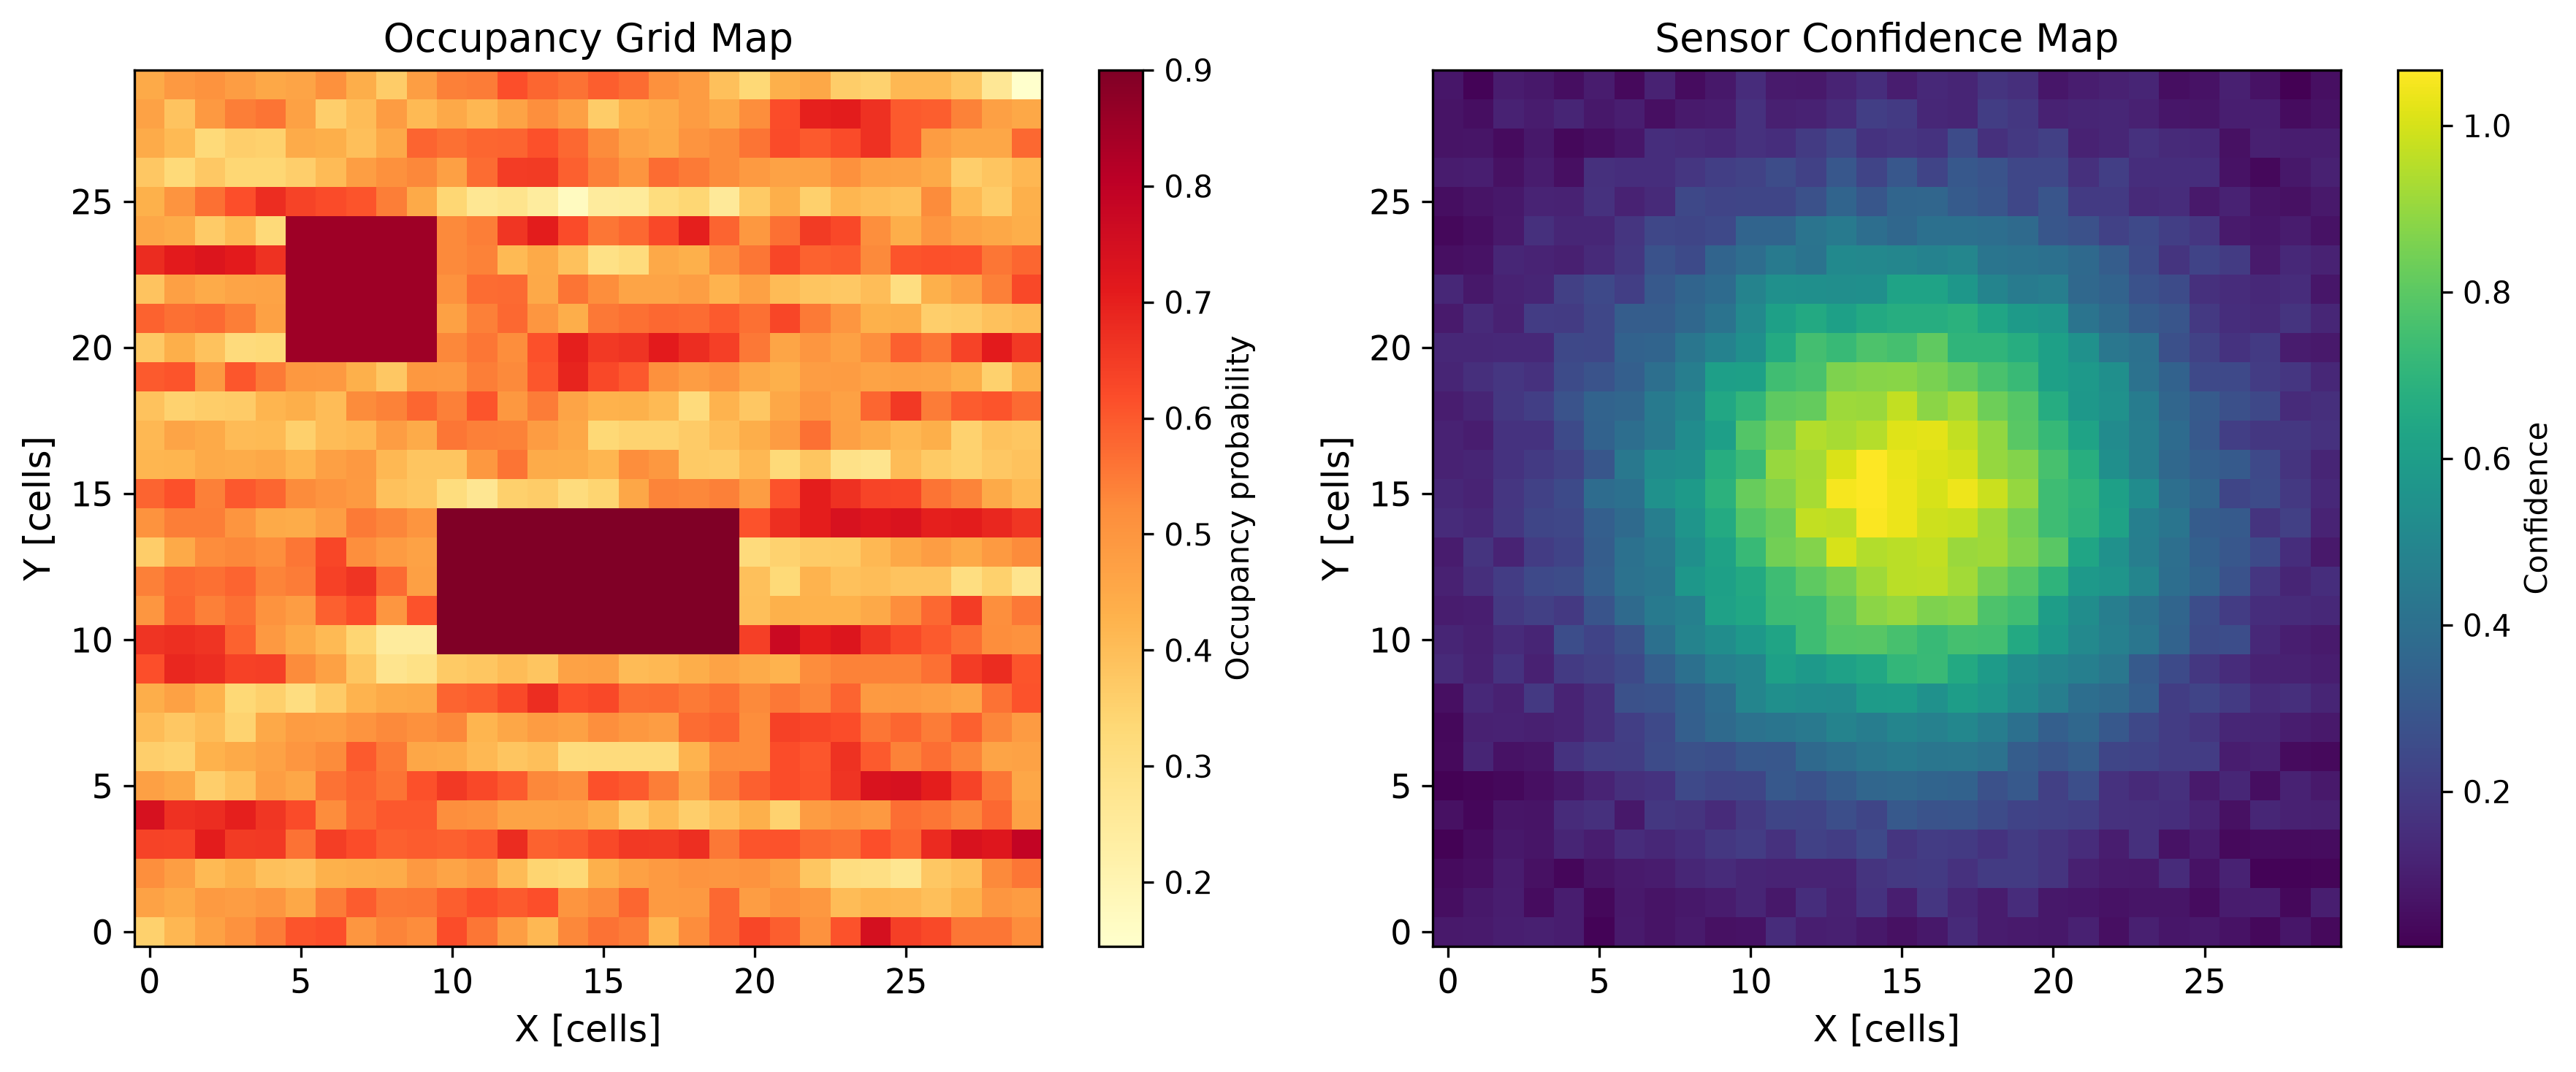
\includegraphics[width=0.95\columnwidth]{figures/fig_sensor_models.png}
    \caption{מודלי החיישנים במערכת: \en{IMU}, \en{DVL} וסונאר. (Sensor models in the system: IMU, DVL and sonar.)}
    \label{fig:sensor_models}
\end{figure*}

\subsection{מודל רעש משולב}
\label{sec:combined_noise}

מודל הרעש המשולב של המערכת משלב את רעשי כל החיישנים למטריצת שונות משותפת אחת. מטריצה זו משמשת באופטימיזציית גרף הגורמים לשקלול נכון של כל מדידה בהתאם לאמינותה. מודל הרעש המשולב מאפשר למערכת להתמודד עם מצבים שבהם חיישן אחד מספק מדידות רועשות במיוחד, על ידי הפחתת משקלו באופטימיזציה. \citet{Grisetti2010g2o} הראו כי מודל רעש מדויק הוא קריטי לביצועי אופטימיזציית גרף הגורמים.

\begin{equation}
\boldsymbol{\Sigma}_{\text{total}} = \text{blockdiag}(\boldsymbol{\Sigma}_{\text{IMU}}, \boldsymbol{\Sigma}_{\text{DVL}}, \boldsymbol{\Sigma}_{\text{sonar}})
\label{eq:combined_noise}
\end{equation}

משוואה~(\ref{eq:combined_noise}) מציגה את מטריצת הרעש המשולבת, הבנויה כמטריצת בלוקים אלכסונית של מטריצות השונות של כל חיישן. מבנה זה מניח אי-תלות בין רעשי החיישנים השונים, הנחה סבירה עבור חיישנים פיזיקליים נפרדים.

\subsection{השוואה למודלי חיישנים חלופיים}
\label{sec:alternative_models}

קיימות מספר גישות חלופיות למודל חיישנים תת-ימיים. גישת \en{Deep Sensor Models} משתמשת ברשתות עצביות ללמידת מודל החיישן מנתונים, במקום להסתמך על מודל פיזיקלי מפורש. גישה זו יכולה ללכוד אי-ליניאריות מורכבות שאינן מתוארות היטב על ידי מודלים פיזיקליים פשוטים. עם זאת, גישת \en{Deep Sensor Models} דורשת כמויות גדולות של נתוני אימון ועלולה להתקשות בהכללה לתנאים חדשים. במערכת המוצעת, אנו משתמשים במודל פיזיקלי מפורש עם פרמטרים הנלמדים מנתוני כיול, המשלב את יתרונות שתי הגישות.

\subsection{מודל בליעת קול במים}
\label{sec:absorption_model}

מודל בליעת הקול במים הוא מרכיב קריטי במודל הסונאר התת-ימי. בליעת הקול במים תלויה בתדר האות, בטמפרטורת המים, במליחות ובעומק. \citet{Thrun2005ProbRobotics} הראו כי בליעת הקול במים גדלה באופן מעריכי עם התדר, מה שמגביל את הטווח האפקטיבי של סונאר בתדרים גבוהים. במים מלוחים בטמפרטורה של 15°C, מקדם הבליעה הוא כ-0.04 \en{dB/m} בתדר 200 \en{kHz}, ועולה לכ-0.4 \en{dB/m} בתדר 1000 \en{kHz}.

מודל הבליעה משפיע על בחירת תדר הסונאר האופטימלי. תדרים נמוכים (200-500 \en{kHz}) מאפשרים טווח ארוך (עד 100 מטר) אך ברזולוציה נמוכה. תדרים גבוהים (500-1000 \en{kHz}) מאפשרים רזולוציה גבוהה אך בטווח מוגבל (עד 30 מטר). במערכת המוצעת, אנו משתמשים בתדר משתנה בהתאם למרחק המטרה ולדרישות הרזולוציה.

\begin{equation}
I(r) = I_0 \cdot e^{-2\alpha r} \cdot \frac{1}{r^2}
\label{eq:absorption}
\end{equation}

משוואה~(\ref{eq:absorption}) מציגה את מודל בליעת הקול במים, שבו $I_0$ היא עוצמת האות המשודר, $\alpha$ הוא מקדם הבליעה, ו-$r$ הוא המרחק מהרכב למטרה. האיבר $1/r^2$ מייצג את דעיכת העוצמה עקב התפשטות כדורית של גלי הקול.

\subsection{מודל ריבוי נתיבים אקוסטי}
\label{sec:multipath_model}

מודל ריבוי נתיבים אקוסטי (\en{multipath model}) מתאר את התפשטות גלי הקול במספר מסלולים בין הרכב למטרה. בסביבה תת-ימית, גלי קול יכולים להגיע למטרה במספר מסלולים: מסלול ישיר, החזרה מפני המים, החזרה מקרקעית הים, והחזרות מרובות. כל מסלול מאופיין באורך שונה, מה שגורם להדים מרובים באות הנקלט.

\citet{Rihaczek1969MatchedFilter} הראו כי ריבוי נתיבים יכול לגרום לשגיאות מדידה משמעותיות במערכות סונאר, במיוחד בסביבות רדודות. במערכת המוצעת, אנו משתמשים באלגוריתם זיהוי מסלול ישיר המבוסס על השוואת עוצמת ההדים וזמני ההגעה שלהם. ההד בעל העוצמה הגבוהה ביותר והזמן הקצר ביותר מזוהה כמסלול הישיר.

\begin{equation}
\tau_{\text{multipath}} = \frac{1}{c} \l$e$ft( \sqrt{(x - x_f)$$^2 + (y - y_f)^2 + (z + z_f)^2} \right)
\label{eq:multipath}
\end{equation}

משוואה~(\ref{eq:multipath}) מציגה את זמן ההגעה של ההד המוחזר מפני המים, שבו $z$ הוא עומק הרכב ו-$z_f$ הוא עומק המטרה. החזרה מפני המים יוצרת מסלול וירטואלי שבו המטרה משתקפת מעל פני המים. זיהוי מסלולים מרובים מאפשר דחיית הדים מזויפים ושיפור דיוק המדידה.
